\documentclass[border=6pt]{standalone}
\usepackage{tikz}
\usetikzlibrary{arrows.meta,positioning,shapes.geometric,shapes.multipart,calc,fit,backgrounds,decorations.pathreplacing,decorations.markings,automata,chains,matrix,patterns}
\usepackage{circuitikz}
\usepackage{amsmath}
\usepackage{amssymb}
\begin{document}
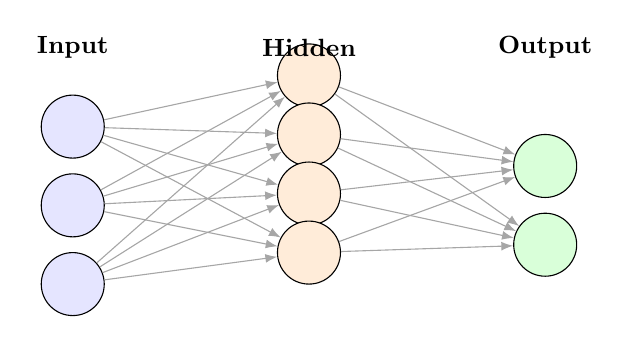
\begin{tikzpicture}[
  neuron/.style={circle, draw, minimum size=0.8cm, fill=blue!10},
  layerlabel/.style={font=\small\bfseries}
]
  \foreach \i in {1,...,3}
    \node[neuron] (I-\i) at (0, -\i) {};
  \node[layerlabel] at (0, 0) {Input};

  \foreach \i in {1,...,4}
    \node[neuron, fill=orange!15] (H-\i) at (3, -\i*0.75+0.4) {};
  \node[layerlabel] at (3, 0) {Hidden};

  \foreach \i in {1,...,2}
    \node[neuron, fill=green!15] (O-\i) at (6, -\i-0.5) {};
  \node[layerlabel] at (6, 0) {Output};

  \foreach \i in {1,...,3}
    \foreach \j in {1,...,4}
      \draw[-{Latex[length=1.5mm]}, gray!70] (I-\i) -- (H-\j);
  \foreach \i in {1,...,4}
    \foreach \j in {1,...,2}
      \draw[-{Latex[length=1.5mm]}, gray!70] (H-\i) -- (O-\j);
\end{tikzpicture}
\end{document}
